\documentclass[main.tex]{subfiles}

\begin{document}

\chapter{Two dimensions}

In the previous chapter, we solved a one-dimensional problem, a penny falling from the Empire State Building.  Now we'll solve a two-dimensional problem, finding the trajectory of a baseball.

\index{baseball}


\section{Spatial vectors}
\label{sect:spacial}

The word ``vector'' means different
things to different people.  In MATLAB, a vector is a matrix that has
either one row or one column.  So far we have used MATLAB vectors to
represent:

\begin{description}

\item[sequences:] A sequence is a set of values identified by
integer indices; it is natural to store the elements of the
sequence as elements of a MATLAB vector.

\item[state vectors:] A state vector is a set of values that
describes the state of a physical system.  When you call
{\tt ode45}, you give it initial conditions in a state
vector.  Then when {\tt ode45} calls your rate function, it
gives you a state vector.

\item[time series:] The results from {\tt ode45} are vectors, {\tt T} and {\tt Y}, that represent a time series, that is, a mapping from the time values in {\tt T} to the values in {\tt Y}.

\end{description}

\index{vector!spatial}
\index{spatial vector}
\index{sequence}
\index{state}
\index{time series}

In this chapter we will see another use of MATLAB vectors: representing
{\bf spatial vectors}.  A spatial vector represents a multidimensional physical quantity like position, velocity, acceleration, or force.

\index{position}

For example, to represent a position in two-dimensional space, we can use a vector with two elements:

\begin{code}
>> P = [3 4]
\end{code}

To interpret this vector, we have to know what coordinate system it is defined in.  Most commonly, we use a Cartesian system where the x-axis points east and the y-axis points north.  In that case {\tt P} represents a point 3 units east and 4 units north of the origin.

\index{Cartesian system}
\index{magnitude}
\index{direction}
\index{Pythagorean theorem}

Spatial vectors represent the magnitude and direction of a physical quantity.  For example, the magnitude of {\tt P} is the distance from the origin to {\tt P}, which is the hypotenuse of the triangle with sides 3 and 4.  We can compute it using the Pythagorean theorem:

\begin{code}
>> sqrt(sum(P.*P))
ans = 5
\end{code}

Or more simply by using the function {\tt norm}, which computes the
``Euclidean norm'' of a vector, which is its magnitude:

\index{norm@{\tt norm}}
\index{Euclidean norm}

\begin{code}
>> norm(P)
ans = 5
\end{code}

There are two ways to get the direction of a vector.  One convention is to compute the angle between the vector and the x-axis:

\begin{code}
>> atan2(P(2), P(1))
ans = 0.9273
\end{code}

In this example, the angle is about \SI{0.9}{\radian}.  But for computational purposes, we often represent direction with a {\bf unit vector}, which is a vector with length 1.  To get a unit vector we can divide a vector by its length:

\begin{code}
function res = hat(V)
    res = V / norm(V)
end
\end{code}
 
This function takes a vector, {\tt V}, and returns a unit vector with the same direction as {\tt V}.  It is called {\tt hat} because in mathematical notation, unit vectors are written with a ``hat'' symbol.  
For example, the unit vector with the same direction as $\vec{P}$ would be written $\uvec{P}$. 

\index{unit vector}
\index{vector!unit}

\section{Adding vectors}

Vectors are particularly useful for representing quantities like force and acceleration because we can add them up without having to think explicitly about direction.

\index{force}
\index{acceleration}

As an example, suppose we have two vectors representing forces:

\begin{code}
>> A = [2, 4];
>> B = [2, -2];
\end{code}

{\tt A} represents a force pulling northeast; {\tt B} represents a force pulling southeast, as shown in Figure~\ref{fig:vector2}

\begin{figure}
\centerline{\includegraphics[height=3in]{book/figs/vector2.eps}}
\caption{The sum of two forces represented by vectors.}
\label{fig:vector2}
\end{figure}

To compute the sum of these forces, all we have to do is add the vectors:

\begin{code}
>> A + B
ans = 4     2
\end{code}

This will come in handy later in the chapter.


\section{ODEs in two dimensions}
\label{sect:projectile}

So far we have used {\tt ode45} to solve a system of first-order equations and a single second-order equation.  Now we'll take one more step, solving a system of second-order equations.

As an example, we'll simulate the flight of a baseball.
Assuming there is no wind and no spin on the ball, it should travel in a vertical plane, so we can think of the system as
two-dimensional, with $x$ representing the horizontal distance
traveled and $y$ representing height or altitude.

\index{baseball}
\index{altitude}
\index{rate function}

Here's a rate function we can use to simulate this system with {\tt ode45}:

\begin{code}
function res = rate_func(t, W)
    P = W(1:2);
    V = W(3:4);

    dPdt = V;
    dVdt = acceleration(t, P, V);

    res = [dPdt; dVdt];
end

function res = acceleration(t, P, V)
    g = 9.8;             % acceleration of gravity in m/s^2
    a_gravity = [0; -g];
    res = a_gravity;
end
\end{code}

The second argument of \verb"rate_func" is understood to be a vector,
{\tt W}, with four elements.  The first two are assigned to {\tt P},
which represents position; the last two are assigned to {\tt V}, which
represents velocity. Both {\tt P} and {\tt V} have two elements
representing the $x$ and $y$ components.

\index{derivative}
\index{velocity}

The goal of the rate function is to compute the derivative of {\tt W}, so the output has to be a vector with four elements, where the first two represent the derivative of {\tt P}  and the last two represent the derivative of {\tt V}.

The derivative of {\tt P} is velocity.  We don't have to compute it; we were given it as part of {\tt W}.

The derivative of {\tt V} is acceleration.  To compute it, we call {\tt acceleration}, which takes as input variables time, position and velocity.  In this example, we don't use any of the input variables, but we will soon.

\index{air resistance}
\index{gravity}

For now we'll ignore air resistance, so the only force on the baseball is gravity.  We represent acceleration due to gravity with a vector that has magnitude {\tt g} and direction along the negative $y$ axis.

Let's assume that a ball is batted from an initial position \SI{1}{\meter} above home plate, with an initial velocity of \SI{30}{\meter\per\second} in the horizontal and \SI{40}{\meter\per\second} in the vertical direction.

\index{initial condition}

Here's how we can call {\tt ode45} with these initial conditions:
 
\begin{code}
    P = [0; 3];       % initial position in m
    V = [40; 30];     % initial velocity in m/s
    W = [P; V];       % initial condition
    
    tspan = [0 8]
    [T, M] = ode45(@rate_func, tspan, W);
\end{code}

{\tt P} and {\tt V} are column vectors because we put semi-colons between the elements.  So {\tt W} is a column vector with four elements.
{\tt tspan} specifies that we want to run the simulation for \SI{6}{\second}.

\index{time span}
\index{output variable}

The output variables from {\tt ode45} are a vector, 
{\tt T}, that contains time values and a matrix, {\tt M}, with four columns: the first two are position; the last two are velocity.

Here's how we can plot position as a function of time:

\begin{code}
	X = M(:, 1);
    Y = M(:, 2);
    
    plot(T, X)
    plot(T, Y)
\end{code}

{\tt X} and {\tt Y} get the first and second columns from {\tt M}, which are the $x$ and $y$ coordinates of position.

\begin{figure}
\centerline{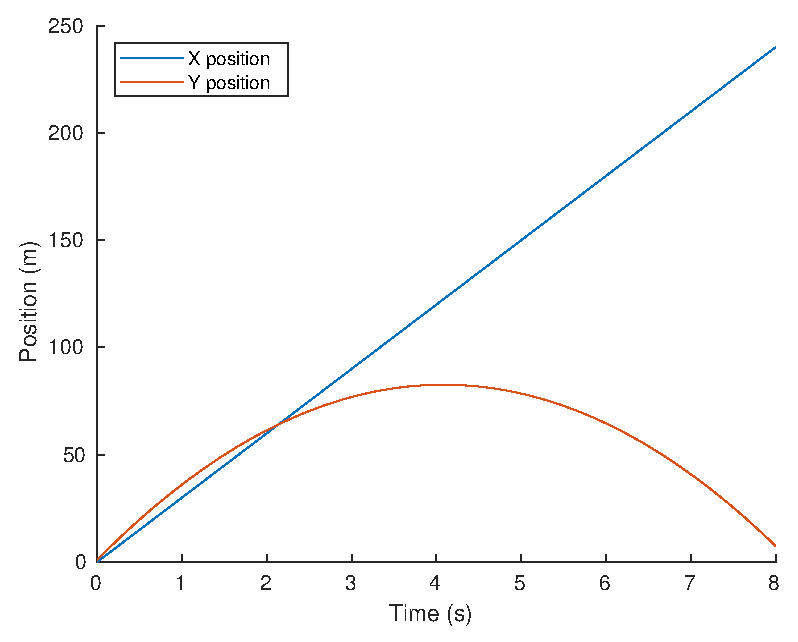
\includegraphics[height=3in]{book/figs/baseball1.eps}}
\caption{Simulated flight of a baseball neglecting drag force.}
\label{fig:baseball1}
\end{figure}

Figure~\ref{fig:baseball1} shows what they look like.  The $x$ coordinate increases linearly because the $x$ velocity is constant.  The $y$ coordinate goes up and down, as we expect.

The simulation ends just before the ball lands, having traveled almost \SI{250}{\meter}.  That's substantially farther than a real baseball would travel, because we have ignored air resistance, or ``drag force''.


\section{Drag force}
\label{sect:drag}

\index{drag}
\index{force!drag}

A simple model for the drag force on a baseball is:

\begin{equation}
    \vec{F_d} = - \frac{1}{2} ~ \rho v^2 C_d A \uvec{V}
\end{equation}

where $\vec{F_d}$ is a vector that represents the force on the baseball
due to drag, 
$\rho$ is the density of air, 
$C_d$ is the drag coefficient, and
$A$ is the cross-sectional area .

\index{drag coefficient}
\index{coefficient!drag}

$\vec{V}$ is the baseball's velocity vector; $v$ is the magnitude of $V$ and $\uvec{V}$ is a unit vector in the same direction as $V$.  The minus sign at the beginning means that the result is in the opposite direction as $V$.

\index{unit vector}

The following function computes the drag force on a baseball:

\begin{code}
 function res = drag_force(V)
    C_d = 0.3;      % dimensionless
    rho = 1.3;      % kg / m^3
    A = 0.0042;     % m^2
    v = norm(V);    % m/s

    res = - 1/2 * C * rho * A * v * V;
end
\end{code}
  
The drag coefficient for a baseball is about 0.3.  
The density of air at sea level is about \SI{1.3}{\kilogram\per\meter\cubed}.
The cross-sectional area of a baseball is \SI{0.0042}{\meter\squared}.

\index{density}
\index{cross-sectional area}

Now we have to update {\tt acceleration} to take drag into account:

\begin{code}
function res = acceleration(t, P, V)
    g = 9.8;                       % acceleration of gravity in m/s^2
    a_gravity = [0; -g];

    m = 0.145;                     % mass in kilograms
    a_drag = drag_force(V) / m;
    res = a_gravity + a_drag;
end
\end{code}

As in Section~\ref{sect:projectile}, {\tt acceleration} represents acceleration due to gravity with a vector that has magnitude {\tt g} and direction along the negative $y$ axis.
But now it also computes drag force, then divides by the mass of the baseball to get acceleration due to drag.
Finally, it adds \verb"a_gravity" and \verb"a_drag" to get the total acceleration of the baseball.

\begin{figure}
\centerline{\includegraphics[height=3in]{book/figs/vector3.eps}}
\caption{Diagram of velocity, $\vec{V}$, acceleration due to drag force, 
$\vec{D}$, acceleration due to gravity, $\vec{G}$, and total acceleration, $\vec{A}$.}
\label{fig:vector3}
\end{figure}

Figure~\ref{fig:vector3} shows these quantities graphically.  Acceleration due to drag, $\vec{D}$, is in the opposite direction of velocity, $\vec{V}$.  Acceleration of gravity, $\vec{G}$, is straight down.  Total acceleration, $\vec{A}$, is the sum of $\vec{D}$ and $\vec{G}$.

\index{acceleration}

\begin{figure}
\centerline{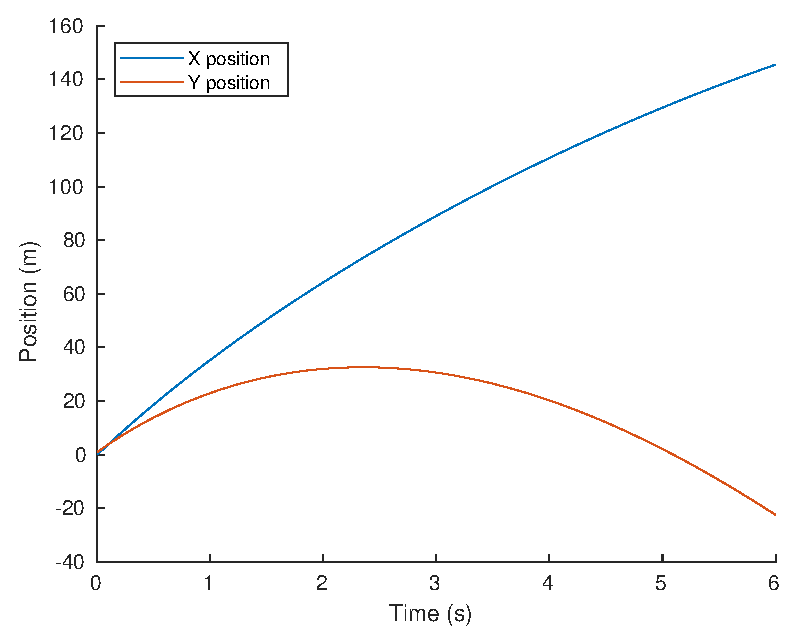
\includegraphics[height=3in]{book/figs/baseball2.eps}}
\caption{Simulated flight of a baseball including drag force.}
\label{fig:baseball2}
\end{figure}

Figure~\ref{fig:baseball2} shows the results from {\tt ode45}.  The ball lands after about \SI{5}{\second}, having traveled less than \SI{150}{\meter}, substantially less than what we got without air resistance, about \SI{250}{\meter}.

This result suggests that ignoring air resistance is not a good choice for modeling a baseball.


\section{What could go wrong?}

What could go wrong?  Well, {\tt vertcat} for one.  To explain
what that means, I'll start with {\bf concatenation}, which is
the operation of joining two matrices into a larger matrix.
``Vertical concatenation'' joins the matrices by stacking them on
top of each other; ``horizontal concatenation'' lays them
side by side.

\index{concatenation}
\index{vertical concatenation}
\index{vertcat@{\tt vertcat}}

Here's an example of horizontal concatenation with row vectors:

\begin{code}
>> x = 1:3
x = 1     2     3

>> y = 4:5
y = 4     5

>> z = [x, y]
z = 1     2     3     4     5
\end{code}

Inside brackets, the comma operator performs horizontal concatenation.
The vertical concatenation operator is the semi-colon.  Here is an
example with matrices:

\index{comma operator}
\index{operator!comma}

\begin{code}
>> X = zeros(2,3)

X =  0     0     0
     0     0     0

>> Y = ones(2,3)

Y =  1     1     1
     1     1     1

>> Z = [X; Y]

Z =  0     0     0
     0     0     0
     1     1     1
     1     1     1
\end{code}

These operations only work if the matrices are the same size along
the dimension where they are glued together.  If not, you get:

\begin{code}
>> a = 1:3

a = 1     2     3

>> b = a'

b =  1
     2
     3

>> c = [a, b]
Error using horzcat
Dimensions of matrices being concatenated are not consistent.

>> c = [a; b]
Error using vertcat
Dimensions of matrices being concatenated are not consistent.
\end{code}

In this example, {\tt a} is a row vector and {\tt b} is a column
vector, so they can't be concatenated in either direction.

Reading the error messages, you probably guessed that {\tt horzcat}
is the function that performs horizontal concatenation, and likewise
with {\tt vertcat} and vertical concatenation.

\index{horzcat@{\tt horzcat}}

In Section~\ref{sect:projectile} we use horizontal concatenation to pack {\tt dRdt} and {\tt dVdt} into the output variable:

\begin{code}
function res = rate_func(t, W)
    P = W(1:2);
    V = W(3:4);

    dPdt = V;
    dVdt = acceleration(t, P, V);

    res = [dPdt; dVdt];
end
\end{code}

As long as {\tt dRdt} and {\tt dVdt} are column vectors,
the semi-colon performs vertical concatenation, and the result is
a column vector with four elements.  But if either of them is a
row vector, that's trouble.

\index{column vector}

{\tt ode45} expects the result from \verb"rate_func" to be a
column vector, so if you are working with {\tt ode45}, it is
probably a good idea to make {\em everything} a column vector.

In general, if you run into problems with {\tt horzcat} and
{\tt vertcat}, use {\tt size} to display the dimensions of the operands,
and make sure you are clear on which way your vectors go.


\section{Glossary}

\begin{description}

\item[spatial vector:] A value that represents a
multidimensional physical quantity like position, velocity,
acceleration or force.

\item[unit vector:] A vector with norm 1, used to indicate
direction.

\item[norm:] The magnitude of a vector.  Sometimes called ``length,''
but not to be confused with the number of elements in a MATLAB
vector.

\item[concatenation:] The operation of joining two matrices end-to-end to
form a new matrix.

\end{description}


\section{Exercises}

\begin{ex}

\index{Boston Red Sox}
\index{density}

When the Boston Red Sox won the World Series in 2007, they played the
Colorado Rockies at their home field in Denver, Colorado.  Find an
estimate of the density of air in the Mile High City.  What effect
does this have on drag?  What effect does it have on the distance the baseball travels?
\end{ex}

\begin{ex}

\index{drag}
\index{air resistance}
\index{coefficient of drag}

The actual drag on a baseball is more complicated than what is
captured by our simple model.  In particular, the drag coefficient
depends on velocity.  You can get some of the details from {\em The
Physics of Baseball}\footnote{Robert K. Adair, Harper Paperbacks, 3rd
Edition, 2002.}; the figure you need is reproduced at \url{https://github.com/AllenDowney/ModSimMatlab/blob/master/code/data/baseball_drag.png}.

Use this data to specify a more realistic model of drag and modify your
program to implement it.  How big is the effect on the distance the baseball travels?
\end{ex}


\begin{ex}
\label{ex:cannon}

\index{cannon}
\index{human cannonball}

According to Wikipedia, the record distance for a human cannonball is 59.05 meters\footnote{See \url{https://en.wikipedia.org/wiki/Human_cannonball}.}.

Modify the example from this chapter to simulate the flight of a human cannonball.  You might have to do some research to find the drag coefficient and cross sectional area for a flying human.

Find the initial velocity (both magnitude and direction) you would need to break this record.  You might have to experiment to find the optimal launch angle.
\end{ex}





% ABD: I am commenting this out for now because the drag equation is
% probably not a good model for this scenario.

%\begin{ex}
%Suppose the baseball lands in a lake, and breaks the water's surface
%with velocity
%
%\begin{equation}
%    v_0 = (25, -25) ~  m/s
%\end{equation}
%
%How long will it take to resurface?
%
%Consider the baseball to be fully submerged when it enters the water. You will need to account for the gravitational force and the drag force (given in equation \eqref{eq:wikidrag}). You will also need to consider the force due to ``buoyancy'' which is given by Archimedes' principle:
%
%\begin{equation}
%    \vec{F_b} = \rho V g ~ \uvec{j}
%\end{equation}
%
%where $\rho$ is the density of the fluid (for water this is $1000 ~ kg /
%m^3$), $V$ is the volume of the fluid displaced (equal to the volume
%of the baseball---take this to be $0.000213 ~ m^3$), and $g$ the
%familiar gravitational constant; $\uvec{j}$ is the unit vector that
%points straight up:
%
%\begin{equation}
%    \uvec{j} = (0, 1)
%\end{equation}
%
%\end{ex}


% chap12


\end{document}
